\section{MVC Framework}
\label{sec:mvc}


\subsection{Structure}

The Model-View-Controller (MVC) framework consists of three different types of components; Views, controllers and models. Each created with a different purpose, see figure \ref{fig:mvc-drawing}

\begin{figure}[h]
	\centering
		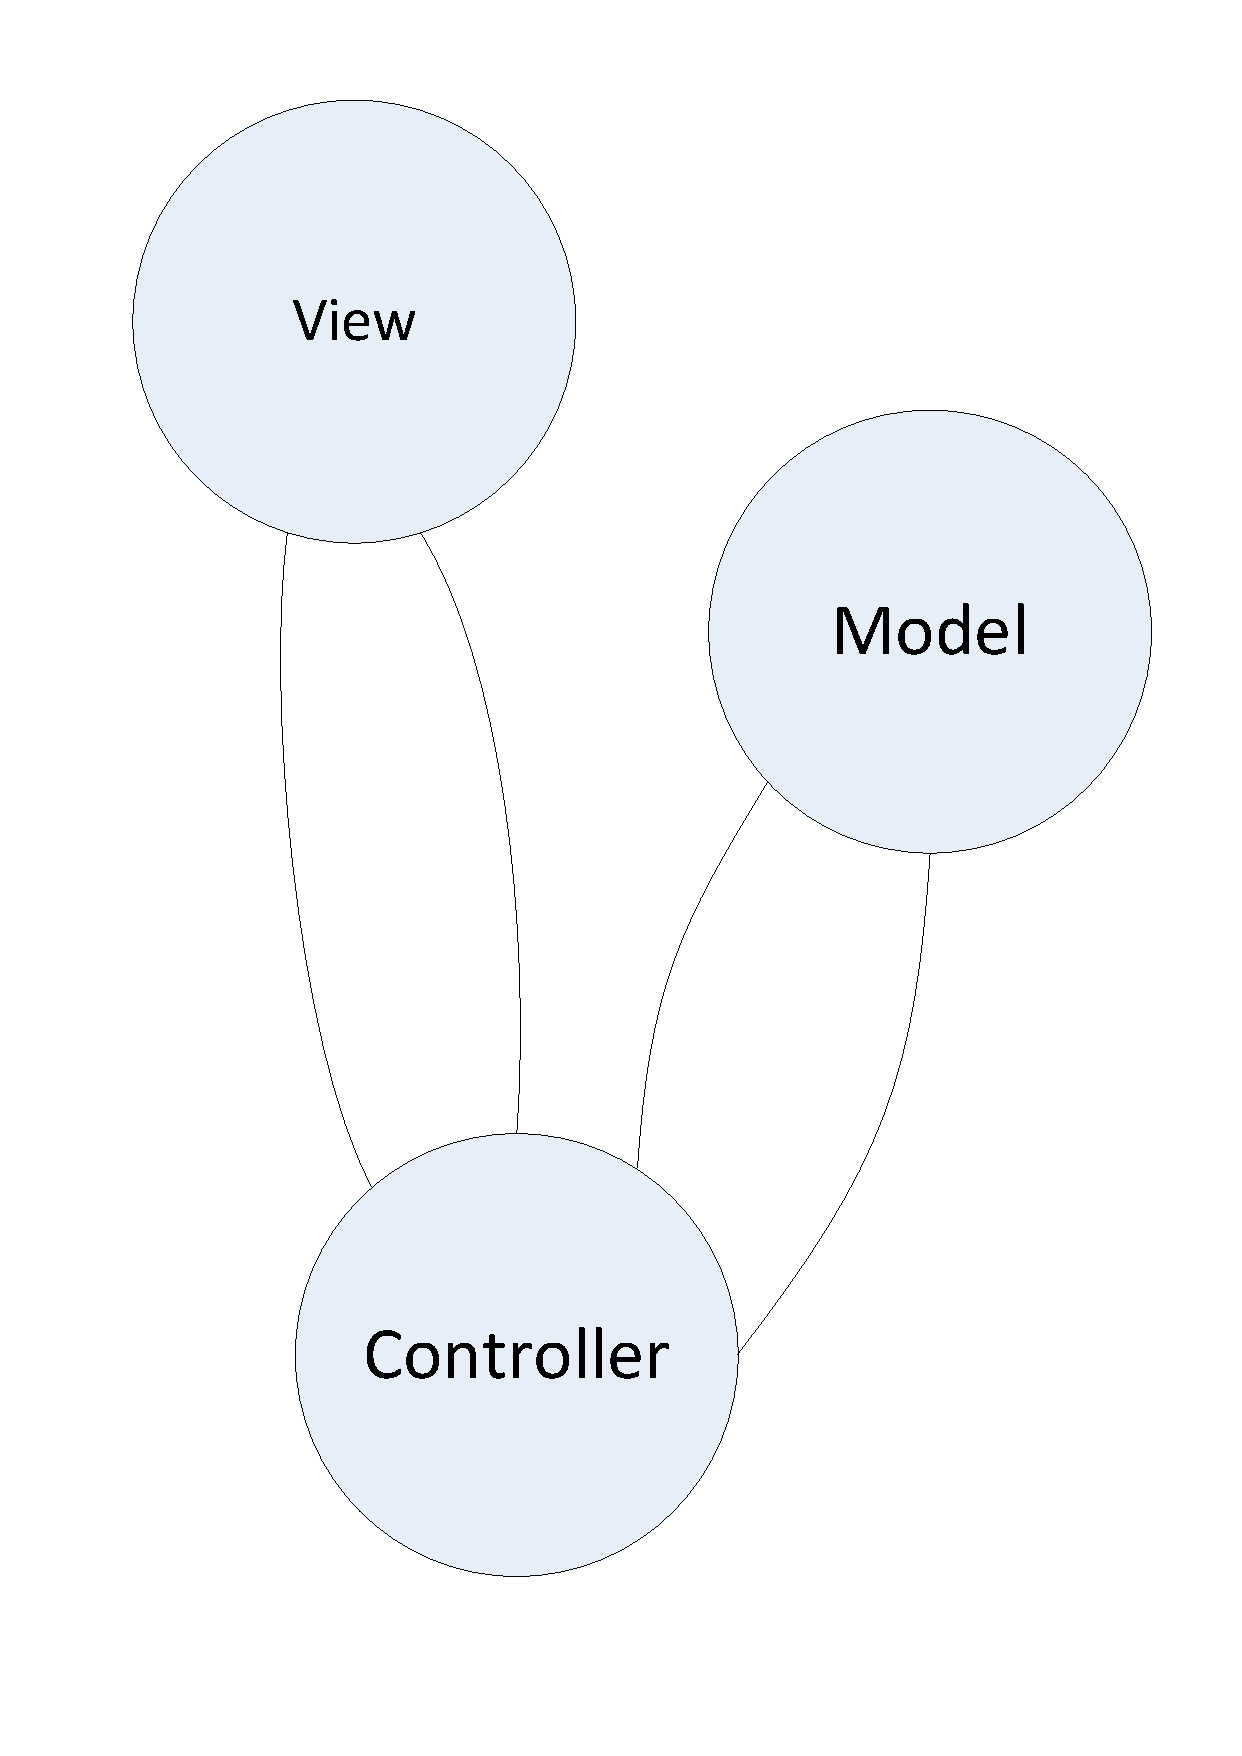
\includegraphics[width=0.90\textwidth]{input/implementation/mvc/MVC.pdf}
	\morscaption{These are the three main components in the MVC}
	\label{fig:mvc-drawing}
\end{figure}


\begin{itemize}
\item Models
\end{itemize}
The models are the components that handle the data domain of the application. Forexample, the model might be mapped to a database, from which it returns data and writes changes.

\begin{itemize}
\item Views
\end{itemize}
The views display the UI and is typically created with data from the model. These views are bascially ordinary (X)HTML pages with the addtion of   C\# or Basic code, to fetch content from the model.

\begin{itemize}
\item Controllers
\end{itemize}
The Controllers reacts to user interaction, and select which view should be rendered. They can also send data with the request, in order to display it in the controller.

Because of the seperation into three independent modules, developers are able to create different parts of the application with different kind of logic, thus enabling them to better manage complexity. It also enables developers to create applications with a high maintainability, because it is easy to alter any of them without effecting the others.

\subsubsection{Displaying actual content}
Another interesting thing about MVC is that there are no actual HTML files. When entering an URL your actually calling mothods in controllers, you can even add parameters if you want. These controllers then redirects you to the correct view. This is possbile beacuse everything is displayed inside of a Master page, which is basically a HTML document, with the addition of content containers. These containers can be created anywehere on the Master page, and act as spaces where views can put their HTML output, the entire page is then created as HTML output, and sent to the browser which requested the page via the URL.

\subsubsection{Data validation}
Client side validation
Server Side validation

\subsubsection{Testing}
When creating web applications with MVC you have the possibility of creating unit tests to thoroughly test your code. These tests can be automatically generated from within Visual Studio, and run as a seperate function, in order to allow the developer to test for all possible inputs. For a more detailed description of Unit-testing in MVC, look in the section \ref{chap:unittest}
